\documentclass{article}

\PassOptionsToPackage{square,comma,numbers,sort&compress}{natbib}

% Keep this line uncommented for the first submission (Peer Review - Anonymous)
%\usepackage{neurips_2024} 

% Uncomment this line for the second submission (Teacher - With Names)
\usepackage[final]{neurips_2024}

\usepackage{graphicx}
\usepackage{caption}
\usepackage{subcaption}
\usepackage[utf8]{inputenc} % allow utf-8 input
\usepackage[T1]{fontenc}    % use 8-bit T1 fonts
\usepackage{hyperref}       % hyperlinks
\usepackage{url}            % simple URL typesetting
\usepackage{booktabs}       % professional-quality tables
\usepackage{amsfonts}       % blackboard math symbols
\usepackage{nicefrac}       % compact symbols for 1/2, etc.
\usepackage{microtype}      % microtypography
\usepackage{xcolor}         % colors
\usepackage{amsmath}        % math support
\usepackage{multirow}       % for multi-row tables

% --- CODE STYLING ---
\definecolor{codegreen}{rgb}{0,0.6,0}
\definecolor{codegray}{rgb}{0.5,0.5,0.5}
\definecolor{codepurple}{rgb}{0.58,0,0.82}
\definecolor{backcolour}{rgb}{0.95,0.95,0.92}

\usepackage{listings}
\lstdefinestyle{mystyle}{
  backgroundcolor=\color{backcolour},
  commentstyle=\color{codegreen},
  keywordstyle=\color{magenta},
  numberstyle=\tiny\color{codegray},
  stringstyle=\color{codepurple},
  basicstyle=\footnotesize\ttfamily,
  breakatwhitespace=false,
  breaklines=true,
  captionpos=b,
  keepspaces=true,
  numbers=left,
  numbersep=2pt,
  showspaces=false,
  showstringspaces=false,
  showtabs=false,
  tabsize=2,
}
\lstset{style=mystyle}

\bibliographystyle{abbrvnat}

\title{Do We Need More Bikes?\\
Project in Statistical Machine Learning}

\author{
  Eric Björling\\
  \AND
  William Degrer\\
  \AND
  Elisa Marie Hurt\\
  \AND
  Upali Bera\\
}

\makeatletter
\renewcommand{\@noticestring}{}
\makeatother

\begin{document}

\maketitle

% (1) ABSTRACT
\begin{abstract}
 The project focuses on the management of the 24/7 public bicycle sharing system, Capital Bikeshare located in Washington D.C. We address the binary classification problem of predicting increased bike demand for the Department of Transportation for better mobility and sustainability. Using a dataset of 1,600 observations, we analyzed temporal and meteorological features to identify when stock increases are needed. We explored several classification methods, including Logistic Regression, Linear and Quadratic Discriminant Analysis, K-Nearest Neighbors, Random Forest, and Gradient Boosting. Gradient Boosting was selected as our production model which achieved a weighted F1-score of 0.92.
  
Number of group members: 4
\end{abstract}

% (2) INTRODUCTION
\section{Introduction}

The Capital Bikeshare system is a cornerstone in the Washington D.C transit network. It offers a sustainable approach compared to using cars for travel. However, the system struggles with a major logistical bottleneck: identifying exactly when and where to move bikes. In this project, we aim to help the District Department of Transportation \cite{uu_course}, by deploying a ML model that predicts whether the stock of bikes needs to be increased (\texttt{high\_bike\_demand}) or not (\texttt{low\_bike\_demand}) at specific hours. Correctly identifying these high demand periods is essential for the department to ensure and maintain bike availability, and by extension also support the city's environmental goals.

% (3) EXPLORATORY DATA ANALYSIS
\section{Exploratory Data Analysis}

\textbf{Feature Exploration:} \\ We analyzed the provided dataset of 1600 samples to better our understanding of the underlying distributions and relationships before modeling. The raw dataset contained 15 potential input features. After preprocessing, we utilized 14 features to predict the binary target variable \texttt{increase\_stock}.

\begin{itemize}
    \item We identified 8 \textbf {numerical features} representing meteorological conditions: \texttt{temp}, \texttt{dew}, \texttt{humidity}, \texttt{precip}, \texttt{snowdepth}, \texttt{windspeed}, \texttt{cloudcover}, and \texttt{visibility}. 
    \item The feature \texttt{snow} (falling snow) was excluded from the model input as we found it to be constant (zero variance) across the training set. However, \texttt{snowdepth} was kept as it contained valid non-zero values.
    \item We identified 6 \textbf{categorical features}. These include the ordinal/cyclical features \texttt{hour\_of\_day}, \texttt{day\_of\_week}, and \texttt{month}. These act as proxies for periodic patterns and commuter behavior. The dataset also includes three binary indicator features: \texttt{holiday}, \texttt{weekday}, and \texttt{summertime}.
\end{itemize}

\textbf{Class Imbalance:} \\ An important finding was the significant class imbalance. "Low Demand" instances outnumber "High Demand" instances by a ratio of approximately 4.5:1. This imbalance is why we decided to use the Weighted F1-Score as our evaluation metric. Accuracy is not a good metric here because a naive model could just guess 'Low Demand' every time and still get a high score.

\textbf{Correlations and Trends:} 
\\Visual inspection confirmed that demand is strongly correlated with \texttt{hour\_of\_day} and \texttt{temp}. Our analysis of the hourly trends revealed a clear commuting pattern where demand increases from morning through afternoon. As shown in Figure \ref{fig:hour_trend}.
\begin{itemize}
    \item The highest demand occurs at 17:00–18:00  with a ~60–75\% high demand rate.
    \item There is a smaller peak around 15:00–16:00.
    \item Late night and early morning hours (00:00–07:00) show nearly no high demand
\end{itemize}

\begin{figure}[h]
  \centering
  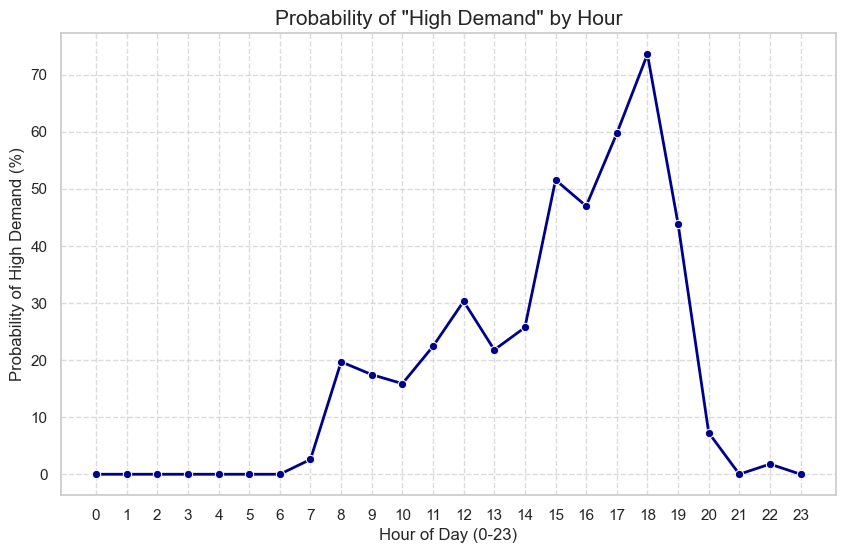
\includegraphics[width=0.5\linewidth]{hour_trend.png} 
  \caption{Average bike demand by hour.}
  \label{fig:hour_trend}
\end{figure}

The weekly data shows several clear trends. As shown in Figure \ref{fig:weekly_trend}.
\begin{itemize}
    \item Highest demand happens on Day 5 (Friday) and Day 6 (Saturday).
    \item Lowest demand happens days 2–3 (Tuesday-Wednesday) which show the lowest probability of high demand.
\end{itemize}

\begin{figure}[h!]
  \centering
  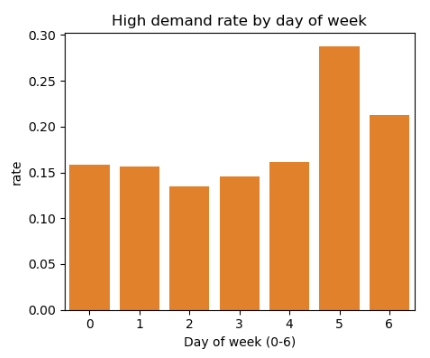
\includegraphics[width=0.7\linewidth]{weekly_trend.png}
  \caption{Average bike demand by weekday.}
  \label{fig:weekly_trend}
\end{figure}

When looking at the monthly data, a seasonal pattern is identified with warmer weather indicating higher demand as shown in Figure \ref{fig:monthly_trend}.
\begin{itemize}
    \item The highest demand happens in months 4, 6, and 9 (April, June, and September) with a ~29–30\% high demand rate.
    \item Winter months (1, 2, 12) have significantly lower demand (~4–12\%).
\end{itemize}

\begin{figure}[h]
  \centering
  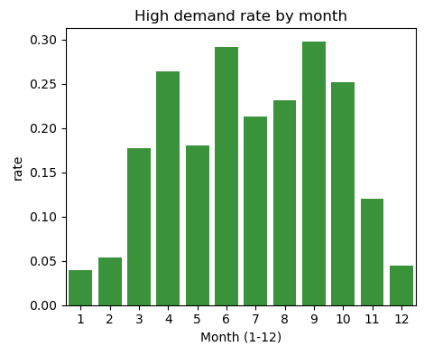
\includegraphics[width=0.7\linewidth]{monthly_trend.png}
  \caption{Average bike demand by month.}
  \label{fig:monthly_trend}
\end{figure}

Our analysis reveals behavioral differences between working days and non-working days. As can be seen from Figure \ref{fig:weekday_holiday_trend}.
\begin{itemize}
    \item \textbf{Weekends (Non-working days):} Show the highest demand with a ~25\% high demand rate. This is significantly higher than regular weekdays.
    \item \textbf{Regular Weekdays:} Show a lower high demand rate of approximately 15\%.
    \item \textbf{Holidays:} Show an intermediate demand level of ~17\%. While slightly higher compared to regular workdays, holidays do not reach the peak demand levels that happens on weekends. There is not a noticeable difference between holidays and non-holidays(18\%).
\end{itemize}

Weekends generate the highest demand, likely due to non-commute activities. Regular weekdays show a lower commuting pattern. The sample size for holidays is small. However, the data shows this category generally requires a stock increase more frequently than average tuesdays.

\begin{figure}[h]
  \centering
  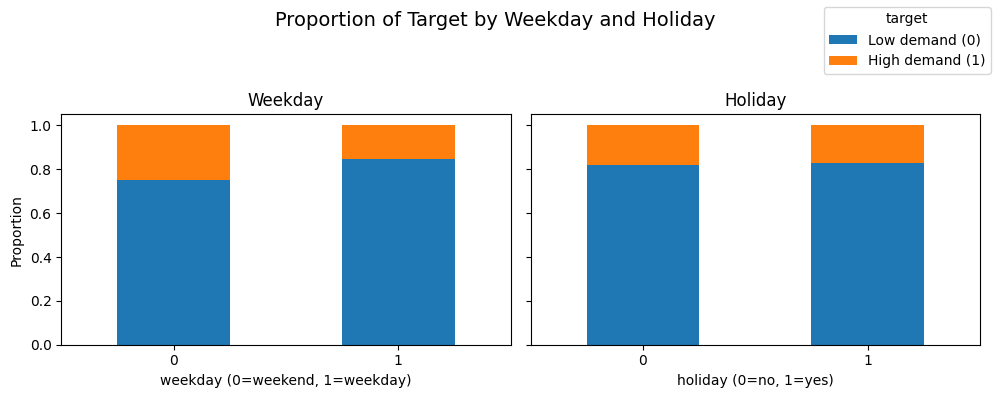
\includegraphics[width=0.7\linewidth]{weekday_holiday.png}
  \caption{Average bike demand by weekday and holiday.}
  \label{fig:weekday_holiday_trend}
\end{figure}

Weather conditions and their correlation with bike demand can be seen from Figure \ref{fig:weather_demand}.

\begin{itemize}
    \item \textbf{Precipitation (Rain/Snow):} Rain acts is in a slight negative correlation with demand (-0.059).
    \item \textbf{Temperature:} There is a strong positive correlation (r = +0.337) between temperature and demand.
    \item \textbf{Humidity:} We observed a strong negative correlation (r = -0.309).
\end{itemize}

Temperature and humidity have a almost linear relationship with demand (positive and negative respectively). Precipitation acts as a binary "switch" that shuts down demand.

\begin{figure}[h]
  \centering
  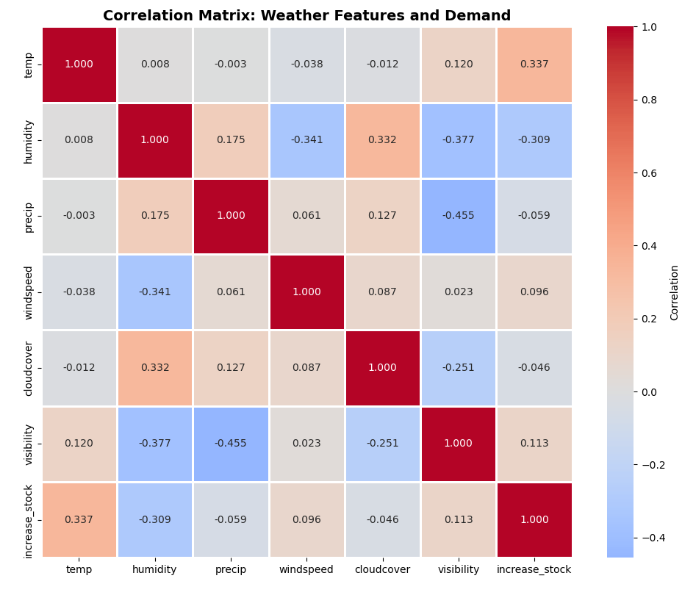
\includegraphics[width=0.7\linewidth]{weather_demand.png}
  \caption{Weather features and demand correlation matrix.}
  \label{fig:weather_demand}
\end{figure}

% (4) MODEL DEVELOPMENT
\section{Model Development}
We implemented the following methods from the classification families, as described in course literature \cite{lindholm2022}\cite{hastie2009}: Logistic Regression, Linear and Quadratic Discriminant Analysis for probabilistic classification, K-Nearest Neighbors (KNN), Random Forest, and Gradient Boosting. We also implemented a naive benchmark using Scikit-learn \cite{scikit-learn}. All models were tuned using cross-validation to prevent overfitting. 
\subsection{Mathematical Descriptions and Methodology}

To address the binary classification of \texttt{increase\_stock}, we implemented and evaluated several models from five distinct families. Each method was chosen to capture different aspects of the relationship between meteorological conditions and bicycle demand.

\textbf{Naive Benchmark:} To establish a baseline for performance, we defined a naive classifier $C_0(x)$ that ignores input features and consistently predicts the most frequent class (\texttt{low\_bike\_demand}) from the training set:
\begin{equation}
    \hat{y} = \text{mode}(\{y_1, ..., y_n\})
\end{equation}
This benchmark is essential for evaluating the actual predictive gain of more complex models, especially given the observed 4.5:1 class imbalance in our dataset.

\textbf{Logistic Regression:} This model estimates the probability of the positive class using the sigmoid function:
\begin{equation}
    P(y=1 \mid x) = \frac{1}{1 + e^{-(\beta_0 + \beta^T x)}},
\end{equation}
where $\beta$ are coefficients learned by maximizing the likelihood of the training data. We chose this method for its high interpretability, as the coefficients directly show how features like \texttt{temp} influence demand. To ensure stable coefficients, all numerical features were scaled using \texttt{StandardScaler}.

\textbf{Linear and Quadratic Discriminant Analysis:} LDA assumes that each class follows a Gaussian distribution with a common covariance matrix $\Sigma$. The discriminant function is:
\begin{equation}
    \delta_k(x) = x^T \Sigma^{-1} \mu_k - \frac{1}{2} \mu_k^T \Sigma^{-1} \mu_k + \log \pi_k
\end{equation}
QDA relaxes this by allowing each class its own covariance matrix $\Sigma_k$, which results in a quadratic decision boundary:
\begin{equation}
    \delta_k(x) = -\frac{1}{2} \log |\Sigma_k| - \frac{1}{2}(x - \mu_k)^T \Sigma_k^{-1}(x - \mu_k) + \log \pi_k
\end{equation}
LDA was implemented as a stable linear baseline, while QDA was motivated by its ability to capture non-linear interactions between weather variables. We used a regularization parameter (\texttt{reg\_param=0.0001}) in QDA to manage potential multicollinearity between features.

\textbf{K-Nearest Neighbors (KNN):} KNN is a non-parametric method that classifies a new observation by identifying the $k$ nearest training samples using the Euclidean distance metric:
\begin{equation}
    d(x, x_i) = \sqrt{\sum_{j=1}^{p} (x_j - x_{ij})^2}
\end{equation}
The advantage of KNN is its flexibility in capturing local demand patterns. In our application, we tuned $k=10$ with distance-weighting to smooth out noise in the meteorological data.

\textbf{Random Forest:} This ensemble method constructs $B$ decorrelated trees using bootstrap aggregating (bagging). For each tree $T_b$, a random subset of $m$ features is used at each split to reduce correlation. The final prediction is a majority vote: 
\begin{equation}
\hat{y} = \text{mode} \{ T_1(x), ..., T_B(x) \}
\end{equation}
Random Forest was chosen for its robustness against overfitting and its inherent ability to handle interactions between categorical proxies and numerical weather data.

\textbf{Gradient Boosting:} Gradient Boosting \cite{xgboost} is an iterative ensemble technique. In each stage $m$, a new tree $h_m(x)$ is fit to the negative gradient of the loss function (pseudo-residuals) of the previous prediction $F_{m-1}(x)$. The model is updated using a learning rate $\nu$: 
\begin{equation}
F_m(x) = F_{m-1}(x) + \nu h_m(x)
\end{equation}
The main advantage of this method is its superior predictive power for complex datasets. We applied it as our final production model, utilizing \texttt{scale\_pos\_weight} to specifically address the imbalance between low and high demand periods.

\subsection{Application and Tuning}

We preprocessed the data by One-Hot Encoding categorical variables and scaling numerical features using \texttt{StandardScaler} for the distance-based and linear models (Logistic Regression, LDA, QDA, KNN) to ensure features with larger scales did not dominate the distance metrics. We utilized Grid Search for hyperparameter tuning, focusing on parameters that control model complexity and prevent overfitting:

\begin{itemize}
    \item \textbf{Logistic Regression:} We tuned the inverse regularization strength $C \in \{0.01, 0.1, 1, 10, 100\}$. $C=1$ was selected to provide a balance between fitting the training data and maintaining a simple model.
    \item \textbf{LDA:} Standard LDA is parameter-free (estimating means/covariance directly). No explicit hyperparameter tuning was applied.
    \item \textbf{QDA:} We tuned the regularization parameter (\texttt{reg\_param}) to handle potential collinearity.
    \item \textbf{KNN:} We tuned $k \in \{1, 3, 5, 7, 10, 15, 20\}$ and weight functions. $k=10$ with uniform weights was chosen as it effectively smoothed local noise in the dataset.
    \item \textbf{Random Forest:} We tuned the model using grid search, optimizing for \texttt{n\_estimators} and \texttt{max\_depth}.
    \item \textbf{Gradient Boosting (XGBoost):} Due to its sensitivity, we performed an extensive grid search over \texttt{learning\_rate}, \texttt{max\_depth}, and \texttt{n\_estimators}. The search aimed to find a low learning rate paired with a sufficient number of trees to minimize the log-loss while handling class imbalance via \texttt{scale\_pos\_weight}. 
\end{itemize}


\subsection{Experimental Evaluation}
We evaluated models using Weighted F1-Score due to the class imbalance.



\begin{table}[h]
    \centering
    \caption{Model comparison based on Weighted F1-Score. The F1 metric was chosen to account for the class imbalance (4.5:1).}
    \label{tab:results}
    \begin{tabular}{lcccc}
        \toprule
        \textbf{Model Family} & \textbf{Weighted F1-Score} & \textbf{Accuracy} & \textbf{Macro recall} & \textbf{Performance Notes} \\
        \midrule
        \textit{Naive Benchmark} & 0.7372 & 0.8187 & 0.5000 & Baseline (Majority Class) \\
        \midrule
        Logistic Regression & 0.8188 & 0.8000 & 0.8175 & Linear model with regularization tuning \\
        LDA & 0.8423 & 0.8562 & 0.6840 & Strong linear baseline \\
        QDA & 0.6498 & 0.6062 & 0.7058 & High recall but lower precision \\
        \midrule
        K-Nearest Neighbors & 0.8016 & 0.8281 & 0.6064 & Sensitive to high dimensionality \\
        \midrule
        Random Forest & 0.9071 & 0.9062 & 0.8219 & Robust, near-top performance \\
        \textbf{Gradient Boosting} & \textbf{0.9192} & \textbf{0.9219} & \textbf{0.8382} & \textbf{Best Model (Selected)} \\
        \bottomrule
    \end{tabular}
\end{table}




\textbf{Performance Analysis:} 
The results in Table \ref{tab:results} highlight the strengths of both linear and ensemble methods.

\begin{itemize}
    \item \textbf{Linear Models:} Both Logistic Regression (F1=0.8188) and LDA (F1=0.8423) performed well, suggesting that a significant portion of the decision boundary can be captured by linear methods. LDA slightly outperformed Logistic Regression, likely due to its assumption of Gaussian-distributed classes.
  \item \textbf{Quadratic Models:} QDA achieved F1 = 0.6498. While QDA typically aims for high recall, the lower overall performance here suggests potential overfitting or violations of the Gaussian assumption. To address potential multicollinearity (e.g., temp vs dew, $r = 0.87$), we investigated whether removing the highly correlated dew feature would improve performance. We found that removing dew decreased performance: F1 declined from 0.6498 to 0.6021. These results indicate that despite its high correlation with temperature, dew retains independent predictive value. The regularization parameter ($\text{reg\_param} = 0.0001$) effectively manages multicollinearity without requiring feature removal.
  
  
  
    \item \textbf{Success of Ensembles:} Gradient Boosting achieved the highest F1-score (0.9192). The Feature Importance plot (Figure \ref{fig:features}) identifies \textbf{hour\_of\_day} and \textbf{visibility} as dominant drivers. This suggests the model leverages the non-linear interaction between specific times of day and favorable weather conditions.
\end{itemize}


While we compared all models on weighted F1-Score, our selected Gradient Boosting model also achieved a global accuracy of 92\% and a weighted precision of 92\% which confirms it is not just guessing the majority class.

\begin{figure}[h]
  \centering
  \begin{minipage}{0.48\textwidth}
    \centering
    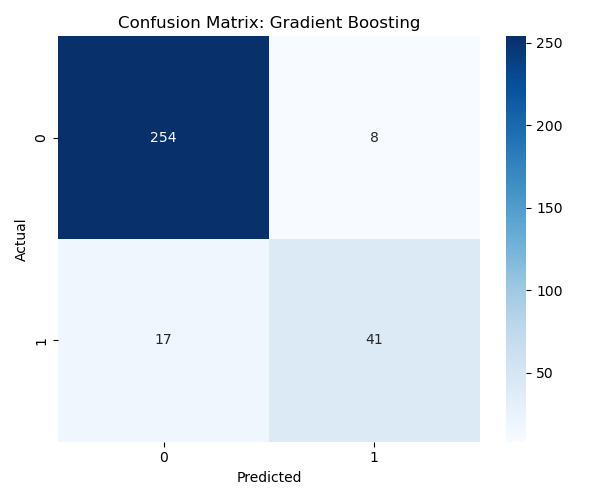
\includegraphics[width=\linewidth]{confusion_matrix.png}
    \caption{Confusion Matrix (Gradient Boosting). The model demonstrates a balanced capability to identify high demand periods.}
    \label{fig:confusion}
  \end{minipage}\hfill
  \begin{minipage}{0.48\textwidth}
    \centering
    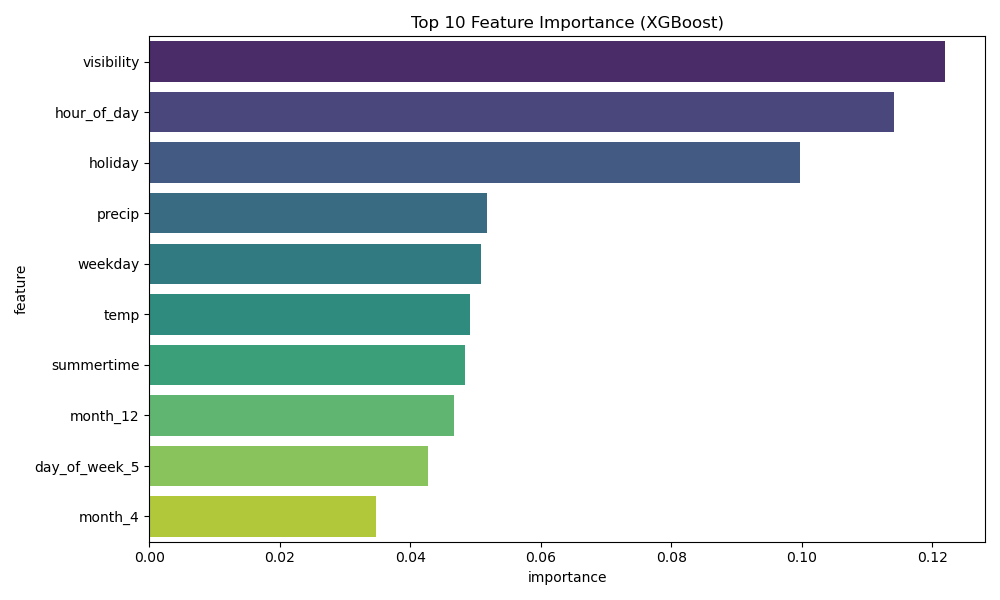
\includegraphics[width=\linewidth]{feature_importance.png}
    \caption{Top 10 Feature Importance (XGBoost). Visibility and hour of day are the strongest predictors.}
    \label{fig:features}
  \end{minipage}
\end{figure}

\subsection{Model Selection}
We selected \textbf{Gradient Boosting} as our production model because it achieved the highest Weighted F1-Score (0.9192). This ensemble method was motivated by its inherent ability to capture non-linear interactions between temporal variables and weather conditions which linear models partially missed. Furthermore it provided better stability against the multicollinearity issues that hindered the QDA model.

% (5) CONCLUSION

\section{Conclusion}
We successfully developed a machine learning pipeline to predict bike sharing demand in Washington, D.C. Our analysis demonstrated that demand is driven by both linear and non-linear interactions between temporal features (hour of day, season) and weather conditions (temperature, humidity).

Linear models - specifically Logistic Regression  and LDA - provided good baselines and captured a substantial portion of the underlying patterns. However, ensemble methods, particularly Gradient Boosting, achieved superior performance with a weighted F1-score of 0.9192, indicating that non-linear relationships and feature interactions are important for accurate demand prediction.


\begin{ack}
We acknowledge the course instructors for the guidance and the provided dataset \cite{uu_course}.
\end{ack}

% --- REFERENCES ---
\bibliographystyle{plainnat} 
\bibliography{ref}           

% CHECKLIST & APPENDIX

\appendix
\section{Appendix: Code}
\lstinputlisting[language=Python]{code.py}

\end{document}